% Options for packages loaded elsewhere
\PassOptionsToPackage{unicode}{hyperref}
\PassOptionsToPackage{hyphens}{url}
%
\documentclass[
]{article}
\usepackage{amsmath,amssymb}
\usepackage{lmodern}
\usepackage{iftex}
\ifPDFTeX
  \usepackage[T1]{fontenc}
  \usepackage[utf8]{inputenc}
  \usepackage{textcomp} % provide euro and other symbols
\else % if luatex or xetex
  \usepackage{unicode-math}
  \defaultfontfeatures{Scale=MatchLowercase}
  \defaultfontfeatures[\rmfamily]{Ligatures=TeX,Scale=1}
\fi
% Use upquote if available, for straight quotes in verbatim environments
\IfFileExists{upquote.sty}{\usepackage{upquote}}{}
\IfFileExists{microtype.sty}{% use microtype if available
  \usepackage[]{microtype}
  \UseMicrotypeSet[protrusion]{basicmath} % disable protrusion for tt fonts
}{}
\makeatletter
\@ifundefined{KOMAClassName}{% if non-KOMA class
  \IfFileExists{parskip.sty}{%
    \usepackage{parskip}
  }{% else
    \setlength{\parindent}{0pt}
    \setlength{\parskip}{6pt plus 2pt minus 1pt}}
}{% if KOMA class
  \KOMAoptions{parskip=half}}
\makeatother
\usepackage{xcolor}
\usepackage[margin=1in]{geometry}
\usepackage{color}
\usepackage{fancyvrb}
\newcommand{\VerbBar}{|}
\newcommand{\VERB}{\Verb[commandchars=\\\{\}]}
\DefineVerbatimEnvironment{Highlighting}{Verbatim}{commandchars=\\\{\}}
% Add ',fontsize=\small' for more characters per line
\usepackage{framed}
\definecolor{shadecolor}{RGB}{248,248,248}
\newenvironment{Shaded}{\begin{snugshade}}{\end{snugshade}}
\newcommand{\AlertTok}[1]{\textcolor[rgb]{0.94,0.16,0.16}{#1}}
\newcommand{\AnnotationTok}[1]{\textcolor[rgb]{0.56,0.35,0.01}{\textbf{\textit{#1}}}}
\newcommand{\AttributeTok}[1]{\textcolor[rgb]{0.77,0.63,0.00}{#1}}
\newcommand{\BaseNTok}[1]{\textcolor[rgb]{0.00,0.00,0.81}{#1}}
\newcommand{\BuiltInTok}[1]{#1}
\newcommand{\CharTok}[1]{\textcolor[rgb]{0.31,0.60,0.02}{#1}}
\newcommand{\CommentTok}[1]{\textcolor[rgb]{0.56,0.35,0.01}{\textit{#1}}}
\newcommand{\CommentVarTok}[1]{\textcolor[rgb]{0.56,0.35,0.01}{\textbf{\textit{#1}}}}
\newcommand{\ConstantTok}[1]{\textcolor[rgb]{0.00,0.00,0.00}{#1}}
\newcommand{\ControlFlowTok}[1]{\textcolor[rgb]{0.13,0.29,0.53}{\textbf{#1}}}
\newcommand{\DataTypeTok}[1]{\textcolor[rgb]{0.13,0.29,0.53}{#1}}
\newcommand{\DecValTok}[1]{\textcolor[rgb]{0.00,0.00,0.81}{#1}}
\newcommand{\DocumentationTok}[1]{\textcolor[rgb]{0.56,0.35,0.01}{\textbf{\textit{#1}}}}
\newcommand{\ErrorTok}[1]{\textcolor[rgb]{0.64,0.00,0.00}{\textbf{#1}}}
\newcommand{\ExtensionTok}[1]{#1}
\newcommand{\FloatTok}[1]{\textcolor[rgb]{0.00,0.00,0.81}{#1}}
\newcommand{\FunctionTok}[1]{\textcolor[rgb]{0.00,0.00,0.00}{#1}}
\newcommand{\ImportTok}[1]{#1}
\newcommand{\InformationTok}[1]{\textcolor[rgb]{0.56,0.35,0.01}{\textbf{\textit{#1}}}}
\newcommand{\KeywordTok}[1]{\textcolor[rgb]{0.13,0.29,0.53}{\textbf{#1}}}
\newcommand{\NormalTok}[1]{#1}
\newcommand{\OperatorTok}[1]{\textcolor[rgb]{0.81,0.36,0.00}{\textbf{#1}}}
\newcommand{\OtherTok}[1]{\textcolor[rgb]{0.56,0.35,0.01}{#1}}
\newcommand{\PreprocessorTok}[1]{\textcolor[rgb]{0.56,0.35,0.01}{\textit{#1}}}
\newcommand{\RegionMarkerTok}[1]{#1}
\newcommand{\SpecialCharTok}[1]{\textcolor[rgb]{0.00,0.00,0.00}{#1}}
\newcommand{\SpecialStringTok}[1]{\textcolor[rgb]{0.31,0.60,0.02}{#1}}
\newcommand{\StringTok}[1]{\textcolor[rgb]{0.31,0.60,0.02}{#1}}
\newcommand{\VariableTok}[1]{\textcolor[rgb]{0.00,0.00,0.00}{#1}}
\newcommand{\VerbatimStringTok}[1]{\textcolor[rgb]{0.31,0.60,0.02}{#1}}
\newcommand{\WarningTok}[1]{\textcolor[rgb]{0.56,0.35,0.01}{\textbf{\textit{#1}}}}
\usepackage{longtable,booktabs,array}
\usepackage{calc} % for calculating minipage widths
% Correct order of tables after \paragraph or \subparagraph
\usepackage{etoolbox}
\makeatletter
\patchcmd\longtable{\par}{\if@noskipsec\mbox{}\fi\par}{}{}
\makeatother
% Allow footnotes in longtable head/foot
\IfFileExists{footnotehyper.sty}{\usepackage{footnotehyper}}{\usepackage{footnote}}
\makesavenoteenv{longtable}
\usepackage{graphicx}
\makeatletter
\def\maxwidth{\ifdim\Gin@nat@width>\linewidth\linewidth\else\Gin@nat@width\fi}
\def\maxheight{\ifdim\Gin@nat@height>\textheight\textheight\else\Gin@nat@height\fi}
\makeatother
% Scale images if necessary, so that they will not overflow the page
% margins by default, and it is still possible to overwrite the defaults
% using explicit options in \includegraphics[width, height, ...]{}
\setkeys{Gin}{width=\maxwidth,height=\maxheight,keepaspectratio}
% Set default figure placement to htbp
\makeatletter
\def\fps@figure{htbp}
\makeatother
\setlength{\emergencystretch}{3em} % prevent overfull lines
\providecommand{\tightlist}{%
  \setlength{\itemsep}{0pt}\setlength{\parskip}{0pt}}
\setcounter{secnumdepth}{-\maxdimen} % remove section numbering
\ifLuaTeX
  \usepackage{selnolig}  % disable illegal ligatures
\fi
\IfFileExists{bookmark.sty}{\usepackage{bookmark}}{\usepackage{hyperref}}
\IfFileExists{xurl.sty}{\usepackage{xurl}}{} % add URL line breaks if available
\urlstyle{same} % disable monospaced font for URLs
\hypersetup{
  pdftitle={Contraceptive Rates For Women of Different Age Groups},
  pdfauthor={Megan Tran},
  hidelinks,
  pdfcreator={LaTeX via pandoc}}

\title{Contraceptive Rates For Women of Different Age Groups}
\author{Megan Tran}
\date{}

\begin{document}
\maketitle

\#Introduction

The dataset used for this research report was downloaded from the
California Health and Human Services Agency (CHHS) Open Data Portal:
\url{https://data.chhs.ca.gov/dataset/contraceptive-care-for-women-use-by-race-ethnicity-contraceptive-type-and-age-group/resource/12a73f54-dcf4-4e38-843c-e988385be69b}.
The Contraceptive Care - All Women measure (CCW), as part of the
Maternal and Infant Health Initiative, Contraceptive Care Quality grant,
was compiled data taken from women ages 15-44 at risk for unintended
pregnancy. The female participants were stratified into two age groups,
those who are 15-20 and those who are 21-44 years old, and six racial
groups. Contraceptive type either fell under the category of long-acting
reversible methods of contraception (LARC), which include birth control
implants and IUDs, or most/moderately effective methods of
contraceptions (M/M), such as oral pills, patches, rings, injectables,
female sterilization, or diaphragms. Data was gathered in the California
for 3 consecutive years, 2014-2016. Furthermore, ``Rate of contraceptive
use'' in the dataset refers to those who use a type of contraceptive
divided by those who are ``eligible'', defined as those that have ever
had sex, are not pregnant or seeking pregnancy, and are fecund.

Research shows that LARC contraceptives are more effective forms of
birth control than M/M methods and are safe for women of all ages to
use. LARC methods could prevent more cases of teenage pregnancy for
young women at risk and who are sexually active. However, M/M methods
are more widely used and may be perceived by the public to be safer
since they don't require surgical insertions of long-term devices into
the body. Young women with inadequate knowledge about sex education and
reproductive health may not have enough information about the different
available contraceptive methods and as a result, be unable to make an
informed decision on the contraceptive type that's right for them.

The research question being explored is if younger women (age 15-20) use
long-acting reversible methods of contraception (LARC) at a lower rate
than older women (age 21-44) and is that trend consistent throughout the
three year period?

\#Methods The role of the California Health and Human Services Agency is
to provide policy leadership and direction to the departments and
programs it oversees, to reduce duplication and fragmentation and
improve coordination among the departments, to ensure programmatic
integrity, and to advance the Governor's priorities on health and human
services issues.

The Agency coordinates the administration of state and federal programs
for public health, health care services, social services, public
assistance, health planning and licensing, and rehabilitation. These
programs touch the lives of millions of California's most needy and
vulnerable residents. The Agency is responsible for balancing the twin
imperatives of providing access to essential health and human services
for California's most disadvantaged and at-risk residents and managing
and controlling costs. The data was collected through administrative
survey measures. The representative sample excluded U.S. women not at
risk of unintended pregnancy because they were infecund for
non-contraceptive reasons, had a live birth in the last 2 months of the
measurement year, or were pregnant or their pregnancy outcome was
unknown at the end of the year(s). Once the exclusions were applied, the
sample included women who were not pregnant at any point in the 3-year
period, those who had a live birth in the first 10 months of the
measurement year(s), and those who had a miscarriage, stillbirth,
ectopic pregnancy, or induced abortion.

Reading in the data:

\begin{Shaded}
\begin{Highlighting}[]
\ControlFlowTok{if}\NormalTok{ (}\SpecialCharTok{!}\FunctionTok{file.exists}\NormalTok{(}\StringTok{"ofp{-}ccw{-}by{-}race{-}ethn\_contra{-}type\_age{-}group\_14{-}16.csv"}\NormalTok{)) \{}
\FunctionTok{download.file}\NormalTok{(}\StringTok{"https://data.chhs.ca.gov/dataset/c2698502{-}d276{-}4e55{-}9057{-}8153e39d21b1/resource/12a73f54{-}dcf4{-}4e38{-}843c{-}e988385be69b/download/ofp{-}ccw{-}by{-}race{-}ethn\_contra{-}type\_age{-}group\_14{-}16.csv"}\NormalTok{, }\StringTok{"ofp{-}ccw{-}by{-}race{-}ethn\_contra{-}type\_age{-}group\_14{-}16.csv"}\NormalTok{, }\AttributeTok{method=}\StringTok{"libcurl"}\NormalTok{, }\AttributeTok{timeout =} \DecValTok{60}\NormalTok{) }
\NormalTok{\}}
\NormalTok{contra }\OtherTok{\textless{}{-}}\NormalTok{ data.table}\SpecialCharTok{::}\FunctionTok{fread}\NormalTok{(}\StringTok{"ofp{-}ccw{-}by{-}race{-}ethn\_contra{-}type\_age{-}group\_14{-}16.csv"}\NormalTok{) }
\end{Highlighting}
\end{Shaded}

First, the number of missing values were checked.

\begin{Shaded}
\begin{Highlighting}[]
\FunctionTok{mean}\NormalTok{(}\FunctionTok{is.na}\NormalTok{(contra))}
\end{Highlighting}
\end{Shaded}

\begin{verbatim}
## [1] 0
\end{verbatim}

There were no missing values in the dataset so there was no need to
remove observations or impute data.

A regular expression was used in order to remove the ``\%'' symbol from
the ``Rate of Contraceptive Use'' column.

\begin{Shaded}
\begin{Highlighting}[]
\NormalTok{contra}\SpecialCharTok{$}\StringTok{\textasciigrave{}}\AttributeTok{Rate of Contraceptive Use}\StringTok{\textasciigrave{}} \OtherTok{\textless{}{-}}\NormalTok{ stringr}\SpecialCharTok{::}\FunctionTok{str\_remove\_all}\NormalTok{(contra}\SpecialCharTok{$}\StringTok{\textasciigrave{}}\AttributeTok{Rate of Contraceptive Use}\StringTok{\textasciigrave{}}\NormalTok{, }\StringTok{"\%"}\NormalTok{)}
\end{Highlighting}
\end{Shaded}

Then the column was changed from a character variable to numeric.

\begin{Shaded}
\begin{Highlighting}[]
\NormalTok{contra}\SpecialCharTok{$}\StringTok{\textasciigrave{}}\AttributeTok{Rate of Contraceptive Use}\StringTok{\textasciigrave{}} \OtherTok{\textless{}{-}} \FunctionTok{as.numeric}\NormalTok{(contra}\SpecialCharTok{$}\StringTok{\textasciigrave{}}\AttributeTok{Rate of Contraceptive Use}\StringTok{\textasciigrave{}}\NormalTok{)}
\end{Highlighting}
\end{Shaded}

There's a wide range between the maximum and minimum rates.

\begin{Shaded}
\begin{Highlighting}[]
\FunctionTok{summary}\NormalTok{(contra}\SpecialCharTok{$}\StringTok{\textasciigrave{}}\AttributeTok{Rate of Contraceptive Use}\StringTok{\textasciigrave{}}\NormalTok{)}
\end{Highlighting}
\end{Shaded}

\begin{verbatim}
##    Min. 1st Qu.  Median    Mean 3rd Qu.    Max. 
##   2.320   6.975  12.270  20.669  35.610  53.310
\end{verbatim}

The average of the rates of contraceptive use was calculated by
contraceptive type, age group, and year. The variable ``avg\_rate'' was
created.

\begin{Shaded}
\begin{Highlighting}[]
\NormalTok{avg\_contra }\OtherTok{\textless{}{-}}\NormalTok{ contra[ , .(}
    \AttributeTok{avg\_rate =} \FunctionTok{mean}\NormalTok{ (}\StringTok{\textasciigrave{}}\AttributeTok{Rate of Contraceptive Use}\StringTok{\textasciigrave{}}\NormalTok{)}
\NormalTok{  ), }
\NormalTok{  by }\OtherTok{=}\NormalTok{ .(}\StringTok{\textasciigrave{}}\AttributeTok{Contraceptive Type}\StringTok{\textasciigrave{}}\NormalTok{, }\StringTok{\textasciigrave{}}\AttributeTok{Age Group}\StringTok{\textasciigrave{}}\NormalTok{, Year)]}

\NormalTok{avg\_contra}
\end{Highlighting}
\end{Shaded}

\begin{verbatim}
##            Contraceptive Type       Age Group Year  avg_rate
##  1: Most/Moderately Effective 15-20 year olds 2014 38.765000
##  2:                      LARC 15-20 year olds 2014  8.635000
##  3: Most/Moderately Effective 21-44 year olds 2014 42.683333
##  4:                      LARC 21-44 year olds 2014  8.290000
##  5:                      LARC 21-44 year olds 2015  6.785714
##  6: Most/Moderately Effective 15-20 year olds 2015 32.613333
##  7:                      LARC 15-20 year olds 2015  5.605000
##  8: Most/Moderately Effective 21-44 year olds 2015 31.471667
##  9: Most/Moderately Effective 15-20 year olds 2016 31.408333
## 10:                      LARC 15-20 year olds 2016  5.156667
## 11: Most/Moderately Effective 21-44 year olds 2016 30.286667
## 12:                      LARC 21-44 year olds 2016  6.576667
\end{verbatim}

\#Preliminary Results

\begin{Shaded}
\begin{Highlighting}[]
\NormalTok{avg\_contra[}\SpecialCharTok{!}\FunctionTok{is.na}\NormalTok{(}\StringTok{\textasciigrave{}}\AttributeTok{avg\_rate}\StringTok{\textasciigrave{}}\NormalTok{)] }\SpecialCharTok{\%\textgreater{}\%} 
  \FunctionTok{ggplot}\NormalTok{()}\SpecialCharTok{+}
  \FunctionTok{geom\_col}\NormalTok{(}\AttributeTok{mapping=}\FunctionTok{aes}\NormalTok{(}\AttributeTok{x=}\StringTok{\textasciigrave{}}\AttributeTok{Contraceptive Type}\StringTok{\textasciigrave{}}\NormalTok{, }\AttributeTok{y=} \StringTok{\textasciigrave{}}\AttributeTok{avg\_rate}\StringTok{\textasciigrave{}}\NormalTok{, }\AttributeTok{fill =} \StringTok{\textasciigrave{}}\AttributeTok{Contraceptive Type}\StringTok{\textasciigrave{}}\NormalTok{)) }\SpecialCharTok{+}
   \FunctionTok{labs}\NormalTok{(}\AttributeTok{title =} \StringTok{"Bar Graphs of Contraceptive Use by Age Group"}\NormalTok{) }\SpecialCharTok{+}
  \FunctionTok{labs}\NormalTok{( }\AttributeTok{y =} \StringTok{"Rate of Contraceptive Use"}\NormalTok{) }\SpecialCharTok{+}
    \FunctionTok{facet\_wrap}\NormalTok{( }\SpecialCharTok{\textasciitilde{}}\StringTok{\textasciigrave{}}\AttributeTok{Age Group}\StringTok{\textasciigrave{}}\NormalTok{)}
\end{Highlighting}
\end{Shaded}

\begin{center}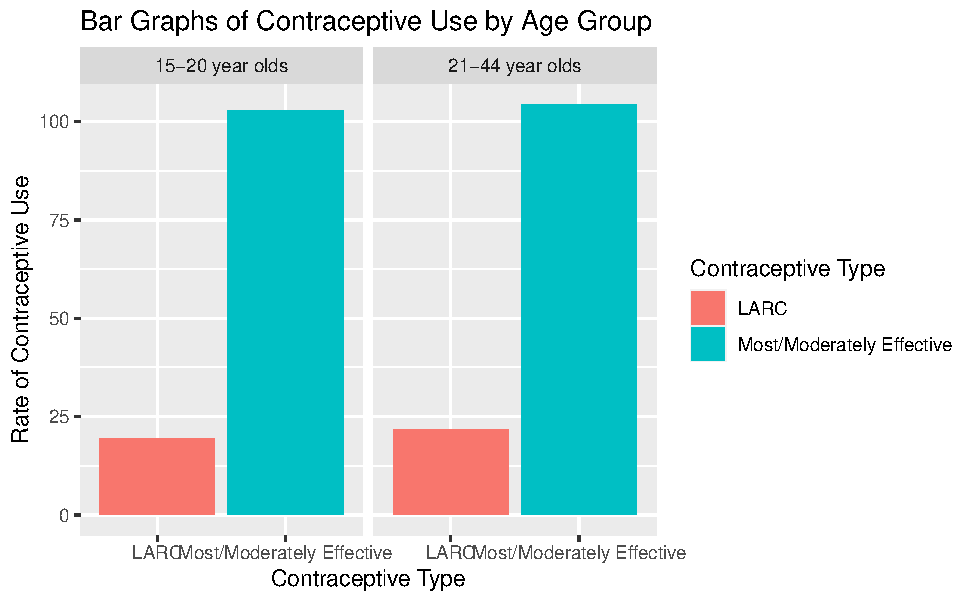
\includegraphics[width=700px]{Report_files/figure-latex/unnamed-chunk-6-1} \end{center}

These bar graphs show the rates of contraceptive use, LARC or
Most/Moderately Effective methods, per age group. The figure shows that
older women use LARC methods at a slightly higher rate. Since these bar
graphs are so similar, I want to see if the graphs look any different
when I split them into years. Perhaps, a different trend will appear.

\begin{Shaded}
\begin{Highlighting}[]
\NormalTok{avg\_contra[}\SpecialCharTok{!}\FunctionTok{is.na}\NormalTok{(}\StringTok{\textasciigrave{}}\AttributeTok{avg\_rate}\StringTok{\textasciigrave{}}\NormalTok{)] }\SpecialCharTok{\%\textgreater{}\%} 
  \FunctionTok{ggplot}\NormalTok{()}\SpecialCharTok{+}
  \FunctionTok{geom\_col}\NormalTok{(}\AttributeTok{mapping=}\FunctionTok{aes}\NormalTok{(}\AttributeTok{x=}\StringTok{\textasciigrave{}}\AttributeTok{Contraceptive Type}\StringTok{\textasciigrave{}}\NormalTok{, }\AttributeTok{y=} \StringTok{\textasciigrave{}}\AttributeTok{avg\_rate}\StringTok{\textasciigrave{}}\NormalTok{, }\AttributeTok{fill =} \StringTok{\textasciigrave{}}\AttributeTok{Contraceptive Type}\StringTok{\textasciigrave{}}\NormalTok{)) }\SpecialCharTok{+}
   \FunctionTok{labs}\NormalTok{(}\AttributeTok{title =} \StringTok{"Bar Graphs of Contraceptive Use by Year and Age Group"}\NormalTok{) }\SpecialCharTok{+}
   \FunctionTok{facet\_wrap}\NormalTok{(Year }\SpecialCharTok{\textasciitilde{}} \StringTok{\textasciigrave{}}\AttributeTok{Age Group}\StringTok{\textasciigrave{}}\NormalTok{, }\AttributeTok{nrow=}\DecValTok{3}\NormalTok{)}
\end{Highlighting}
\end{Shaded}

\begin{center}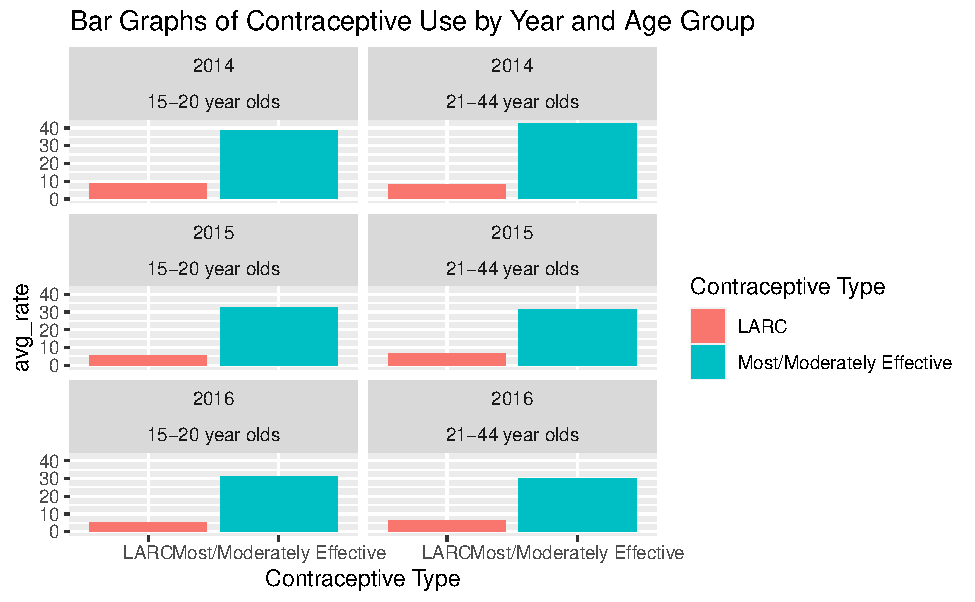
\includegraphics[width=700px]{Report_files/figure-latex/unnamed-chunk-7-1} \end{center}

These bar graphs split the data by year. Interestingly enough, older
women used LARC methods at a lower rate than younger women in 2014. In
the next two years, you can observe that the rates for 15-20 year olds
decreased. These graphs give us a better idea of how the rate
distribution changes for the two age groups over the years. They suggest
that time might be confounder in the association between contraceptive
type and age group since the trend is different for different years.

\begin{Shaded}
\begin{Highlighting}[]
\NormalTok{contra[}\SpecialCharTok{!}\FunctionTok{is.na}\NormalTok{(}\StringTok{\textasciigrave{}}\AttributeTok{Rate of Contraceptive Use}\StringTok{\textasciigrave{}}\NormalTok{)] }\SpecialCharTok{\%\textgreater{}\%} 
  \FunctionTok{ggplot}\NormalTok{()}\SpecialCharTok{+}
  \FunctionTok{geom\_boxplot}\NormalTok{(}\AttributeTok{mapping=}\FunctionTok{aes}\NormalTok{(}\AttributeTok{x=}\StringTok{\textasciigrave{}}\AttributeTok{Contraceptive Type}\StringTok{\textasciigrave{}}\NormalTok{, }\AttributeTok{y=}\StringTok{\textasciigrave{}}\AttributeTok{Rate of Contraceptive Use}\StringTok{\textasciigrave{}}\NormalTok{, }\AttributeTok{fill =} \StringTok{\textasciigrave{}}\AttributeTok{Contraceptive Type}\StringTok{\textasciigrave{}}\NormalTok{)) }\SpecialCharTok{+}
   \FunctionTok{labs}\NormalTok{(}\AttributeTok{title =} \StringTok{"Boxplots of Contraceptive Use by Year and Age Group"}\NormalTok{) }\SpecialCharTok{+} 
    \FunctionTok{facet\_wrap}\NormalTok{(Year }\SpecialCharTok{\textasciitilde{}} \StringTok{\textasciigrave{}}\AttributeTok{Age Group}\StringTok{\textasciigrave{}}\NormalTok{, }\AttributeTok{nrow=}\DecValTok{3}\NormalTok{)}
\end{Highlighting}
\end{Shaded}

\begin{center}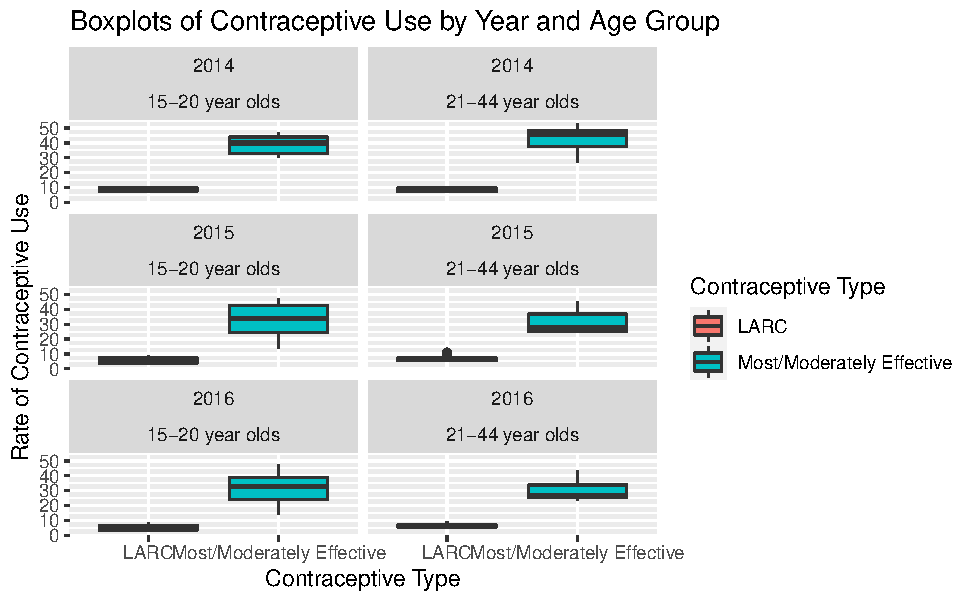
\includegraphics[width=700px]{Report_files/figure-latex/unnamed-chunk-8-1} \end{center}

Again, the boxplots depict the distribution of contraceptive rates by
year, age group, and contraceptive type. Similar to the bar graphs,
these boxplots confirm that the median LARC contraceptive use rates for
younger women are only higher than for older women only in 2014. The
opposite is true for the next two years. There seems to be an outlier
for LARC contraceptive types in 2015 for 21-44 year olds. By examining
the data more closely, we can see that the outlier is not particularly
concerning because it comes from the ``Other Asian/Pacific Islander''
racial group and they consistently have higher rates throughout the
dataset.

\begin{Shaded}
\begin{Highlighting}[]
\NormalTok{database }\OtherTok{\textless{}{-}} \FunctionTok{data.frame}\NormalTok{(}
    \AttributeTok{Year =}\NormalTok{ avg\_contra}\SpecialCharTok{$}\NormalTok{Year, }
   \AttributeTok{Contraceptive\_Type =}\NormalTok{ avg\_contra}\SpecialCharTok{$}\StringTok{\textasciigrave{}}\AttributeTok{Contraceptive Type}\StringTok{\textasciigrave{}}\NormalTok{,}
    \AttributeTok{Age\_Group =}\NormalTok{ avg\_contra}\SpecialCharTok{$}\StringTok{\textasciigrave{}}\AttributeTok{Age Group}\StringTok{\textasciigrave{}}\NormalTok{,}
   \AttributeTok{Average\_Rate\_of\_Contraceptive\_Use =}\NormalTok{ avg\_contra}\SpecialCharTok{$}\NormalTok{avg\_rate}
\NormalTok{ )}
\NormalTok{ knitr}\SpecialCharTok{::}\FunctionTok{kable}\NormalTok{(database, }\AttributeTok{caption =} \StringTok{"Contraceptive Use of Women 2014{-}2016"}\NormalTok{)}
\end{Highlighting}
\end{Shaded}

\begin{longtable}[]{@{}
  >{\raggedleft\arraybackslash}p{(\columnwidth - 6\tabcolsep) * \real{0.0617}}
  >{\raggedright\arraybackslash}p{(\columnwidth - 6\tabcolsep) * \real{0.3210}}
  >{\raggedright\arraybackslash}p{(\columnwidth - 6\tabcolsep) * \real{0.1975}}
  >{\raggedleft\arraybackslash}p{(\columnwidth - 6\tabcolsep) * \real{0.4198}}@{}}
\caption{Contraceptive Use of Women 2014-2016}\tabularnewline
\toprule()
\begin{minipage}[b]{\linewidth}\raggedleft
Year
\end{minipage} & \begin{minipage}[b]{\linewidth}\raggedright
Contraceptive\_Type
\end{minipage} & \begin{minipage}[b]{\linewidth}\raggedright
Age\_Group
\end{minipage} & \begin{minipage}[b]{\linewidth}\raggedleft
Average\_Rate\_of\_Contraceptive\_Use
\end{minipage} \\
\midrule()
\endfirsthead
\toprule()
\begin{minipage}[b]{\linewidth}\raggedleft
Year
\end{minipage} & \begin{minipage}[b]{\linewidth}\raggedright
Contraceptive\_Type
\end{minipage} & \begin{minipage}[b]{\linewidth}\raggedright
Age\_Group
\end{minipage} & \begin{minipage}[b]{\linewidth}\raggedleft
Average\_Rate\_of\_Contraceptive\_Use
\end{minipage} \\
\midrule()
\endhead
2014 & Most/Moderately Effective & 15-20 year olds & 38.765000 \\
2014 & LARC & 15-20 year olds & 8.635000 \\
2014 & Most/Moderately Effective & 21-44 year olds & 42.683333 \\
2014 & LARC & 21-44 year olds & 8.290000 \\
2015 & LARC & 21-44 year olds & 6.785714 \\
2015 & Most/Moderately Effective & 15-20 year olds & 32.613333 \\
2015 & LARC & 15-20 year olds & 5.605000 \\
2015 & Most/Moderately Effective & 21-44 year olds & 31.471667 \\
2016 & Most/Moderately Effective & 15-20 year olds & 31.408333 \\
2016 & LARC & 15-20 year olds & 5.156667 \\
2016 & Most/Moderately Effective & 21-44 year olds & 30.286667 \\
2016 & LARC & 21-44 year olds & 6.576667 \\
\bottomrule()
\end{longtable}

\begin{Shaded}
\begin{Highlighting}[]
\NormalTok{avg\_contra[}\SpecialCharTok{!}\FunctionTok{is.na}\NormalTok{(}\StringTok{\textasciigrave{}}\AttributeTok{avg\_rate}\StringTok{\textasciigrave{}}\NormalTok{)] }\SpecialCharTok{\%\textgreater{}\%} 
  \FunctionTok{ggplot}\NormalTok{()}\SpecialCharTok{+}
\FunctionTok{geom\_col}\NormalTok{(}\AttributeTok{mapping=}\FunctionTok{aes}\NormalTok{(}\AttributeTok{x=}\NormalTok{Year, }\AttributeTok{y=}\NormalTok{ avg\_rate, }\AttributeTok{fill =}\StringTok{"Age Group"}\NormalTok{), }\AttributeTok{position =} \StringTok{"dodge"}\NormalTok{) }\SpecialCharTok{+}
\FunctionTok{facet\_wrap}\NormalTok{( }\SpecialCharTok{\textasciitilde{}} \StringTok{"Contraceptive Type"}\NormalTok{, }\AttributeTok{nrow=}\DecValTok{2}\NormalTok{)}
\end{Highlighting}
\end{Shaded}

\begin{center}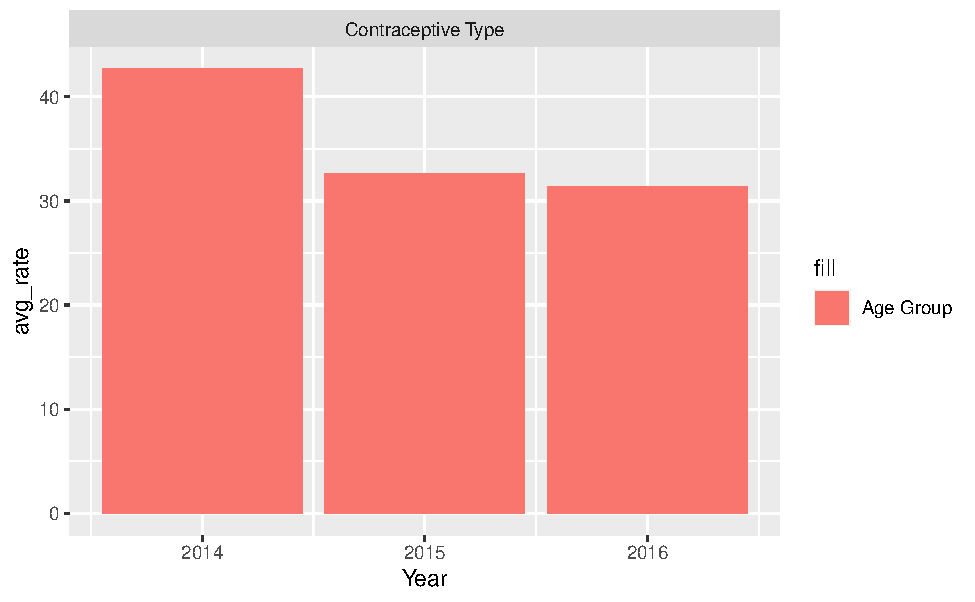
\includegraphics[width=700px]{Report_files/figure-latex/unnamed-chunk-10-1} \end{center}

\begin{Shaded}
\begin{Highlighting}[]
\NormalTok{avg\_contra[}\SpecialCharTok{!}\FunctionTok{is.na}\NormalTok{(}\StringTok{\textasciigrave{}}\AttributeTok{avg\_rate}\StringTok{\textasciigrave{}}\NormalTok{)] }\SpecialCharTok{\%\textgreater{}\%} 
  \FunctionTok{ggplot}\NormalTok{()}\SpecialCharTok{+}
  \FunctionTok{geom\_col}\NormalTok{(}\AttributeTok{mapping=}\FunctionTok{aes}\NormalTok{(}\AttributeTok{x=}\NormalTok{ Year, }\AttributeTok{y=}\NormalTok{ avg\_rate, }\AttributeTok{fill =} \StringTok{\textasciigrave{}}\AttributeTok{Age Group}\StringTok{\textasciigrave{}}\NormalTok{), }\AttributeTok{position =} \StringTok{"dodge"}\NormalTok{) }\SpecialCharTok{+}
\FunctionTok{facet\_wrap}\NormalTok{( }\SpecialCharTok{\textasciitilde{}} \StringTok{\textasciigrave{}}\AttributeTok{Contraceptive Type}\StringTok{\textasciigrave{}}\NormalTok{, }\AttributeTok{nrow=}\DecValTok{2}\NormalTok{)}
\end{Highlighting}
\end{Shaded}

\begin{center}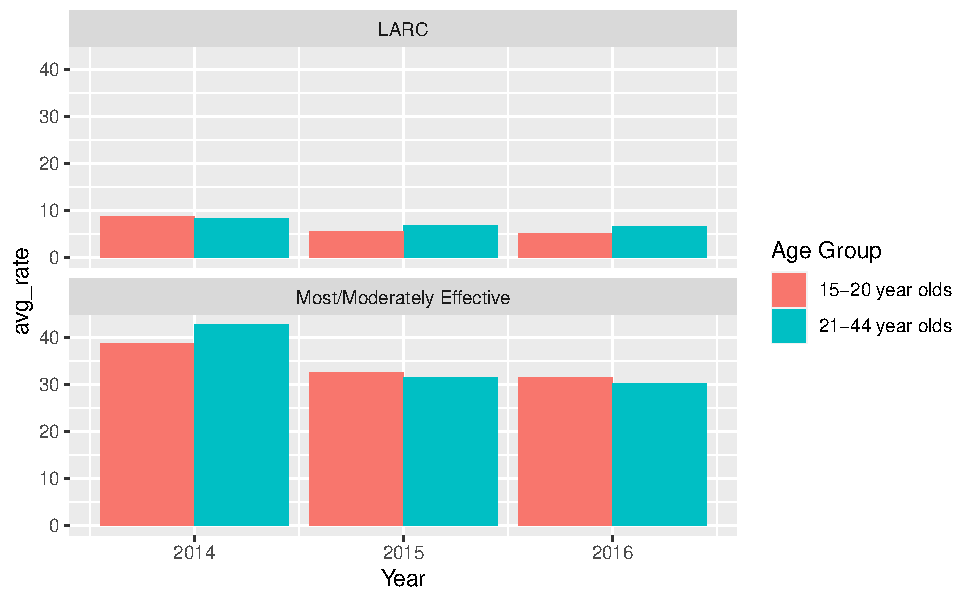
\includegraphics[width=700px]{Report_files/figure-latex/unnamed-chunk-11-1} \end{center}

\#Conclusion

Although statistical analyses should be conducted in order to determine
a more accurate conclusion, we can look at the figures and table to
reach a preliminary conclusion. In reference to the formulated research
question, younger women do indeed use LARC contraceptive methods at a
lower rate than older women, but this was not true for all 3 years,
2014-2016. In 2014, younger women actually had higher rates for LARC
contraceptive use. More research should be conducted as to why there was
a change between 2014 and 2015 and if the trend has held the same past
2016. Introducing LARC contraceptive methods to younger women could
reduce unwanted pregnancies and offer alternative, long-term
contraception options. It's important to note the limitations of the
data. The measure doesn't account for several aspects of women's risk of
unintended pregnancy including sexual experience, pregnancy
intention,sterilization or LARC insertion in a year preceding the
measurement year, and infertility for non-contraceptive reasons. These
factors surely affect the rates reported in the data and future research
should factor in these reasons.

\hypertarget{the-graph-that-i-fixed-from-midterm}{%
\section{the graph that I fixed from
midterm}\label{the-graph-that-i-fixed-from-midterm}}

\begin{Shaded}
\begin{Highlighting}[]
\NormalTok{avg\_contra2 }\OtherTok{\textless{}{-}}\NormalTok{ avg\_contra[ , .(}
    \AttributeTok{avg =} \FunctionTok{mean}\NormalTok{ (avg\_rate)}
\NormalTok{  ), }
\NormalTok{  by }\OtherTok{=}\NormalTok{ .(}\StringTok{\textasciigrave{}}\AttributeTok{Age Group}\StringTok{\textasciigrave{}}\NormalTok{, }\StringTok{\textasciigrave{}}\AttributeTok{Contraceptive Type}\StringTok{\textasciigrave{}}\NormalTok{)]}

\NormalTok{avg\_contra2}
\end{Highlighting}
\end{Shaded}

\begin{verbatim}
##          Age Group        Contraceptive Type       avg
## 1: 15-20 year olds Most/Moderately Effective 34.262222
## 2: 15-20 year olds                      LARC  6.465556
## 3: 21-44 year olds Most/Moderately Effective 34.813889
## 4: 21-44 year olds                      LARC  7.217460
\end{verbatim}

\begin{Shaded}
\begin{Highlighting}[]
\NormalTok{avg\_contra2 }\SpecialCharTok{\%\textgreater{}\%} 
  \FunctionTok{ggplot}\NormalTok{()}\SpecialCharTok{+}
  \FunctionTok{geom\_col}\NormalTok{(}\AttributeTok{mapping=}\FunctionTok{aes}\NormalTok{(}\AttributeTok{x=}\StringTok{\textasciigrave{}}\AttributeTok{Contraceptive Type}\StringTok{\textasciigrave{}}\NormalTok{, }\AttributeTok{y=}\NormalTok{ avg, }\AttributeTok{fill =} \StringTok{\textasciigrave{}}\AttributeTok{Contraceptive Type}\StringTok{\textasciigrave{}}\NormalTok{)) }\SpecialCharTok{+}
   \FunctionTok{labs}\NormalTok{(}\AttributeTok{title =} \StringTok{"Bar Graphs of Contraceptive Use by Age Group"}\NormalTok{) }\SpecialCharTok{+}
  \FunctionTok{labs}\NormalTok{( }\AttributeTok{y =} \StringTok{"Rate of Contraceptive Use"}\NormalTok{) }\SpecialCharTok{+}
    \FunctionTok{facet\_wrap}\NormalTok{( }\SpecialCharTok{\textasciitilde{}}\StringTok{\textasciigrave{}}\AttributeTok{Age Group}\StringTok{\textasciigrave{}}\NormalTok{)}
\end{Highlighting}
\end{Shaded}

\begin{center}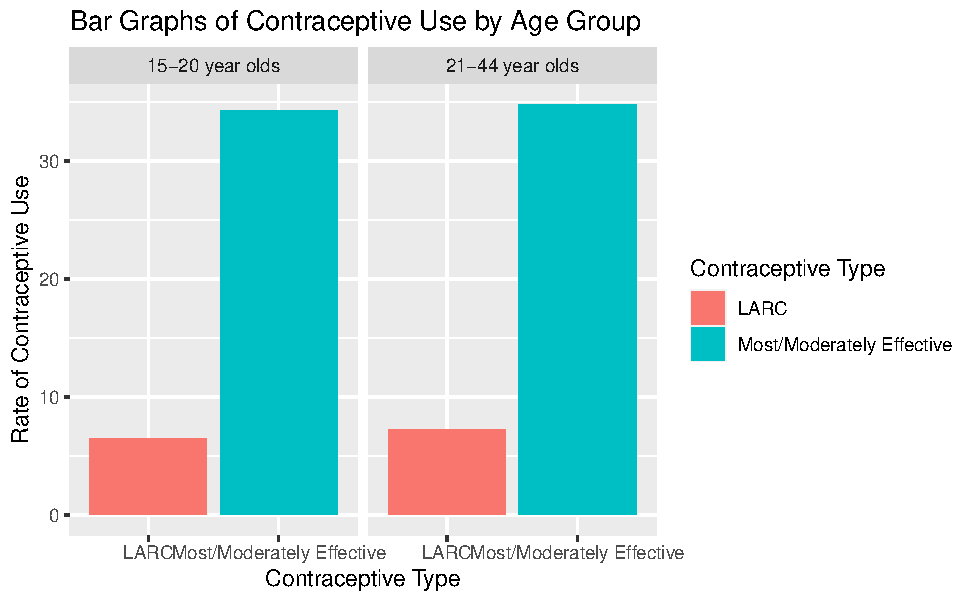
\includegraphics[width=700px]{Report_files/figure-latex/unnamed-chunk-13-1} \end{center}

\end{document}
